\documentclass[12pt,a4paper]{report}

% Packages
\usepackage[utf8]{inputenc}
\usepackage[T1]{fontenc}
\usepackage[polish]{babel}
\usepackage{graphicx}
\usepackage{amsmath}
\usepackage{geometry}
\usepackage[hidelinks]{hyperref}
\usepackage{booktabs}
\usepackage{minted}
\usepackage{titlesec}
\usepackage{csvsimple}
\usepackage{pgfplotstable}
\usepackage{xcolor}
\usepackage{algorithm}
\usepackage{algpseudocode}
\usepackage{pgfplots}
\pgfplotsset{compat=1.18}


% Tłumaczenia nazw
\floatname{algorithm}{Algorytm}

% Tłumaczenia słów kluczowych
\algrenewcommand\algorithmicrequire{\textbf{Dane wejściowe:}}
\algrenewcommand\algorithmicensure{\textbf{Dane wyjściowe:}}

\algrenewcommand\algorithmicif{\textbf{jeżeli}}
\algrenewcommand\algorithmicthen{\textbf{wtedy}}
\algrenewcommand\algorithmicelse{\textbf{w przeciwnym razie}}

\algrenewcommand\algorithmicfor{\textbf{dla}}
\algrenewcommand\algorithmicdo{\textbf{wykonuj}}

\algrenewcommand\algorithmicwhile{\textbf{dopóki}}

\algrenewcommand\algorithmicrepeat{\textbf{powtarzaj}}
\algrenewcommand\algorithmicuntil{\textbf{aż}}

\algrenewcommand\algorithmicreturn{\textbf{zwróć}}

\algrenewcommand\algorithmicend{\textbf{koniec}}

\usemintedstyle{monokai}

\pgfplotstableset{
    highlight/.style={
        postproc cell content/.append code={
            \ifnum\pgfplotstablerow=0
                \pgfkeysalso{@cell content=\cellcolor{gray!20}\pgfplotsretval}%
            \fi
        }
    }
}

\titleformat{\chapter}[hang]
  {\normalfont\huge\bfseries}{\thechapter}{1em}{}
\titlespacing*{\chapter}{0pt}{-20pt}{40pt}

\AtBeginDocument{
  \addtolength{\leftskip}{1.5em}
  \addtolength{\rightskip}{1.5em}
}

% Page margins
\geometry{
    left=15mm,
    right=15mm,
    top=15mm,
    bottom=15mm
}

\title{Techniki Inteligentnej Analizy Danych\\[0.5em]\large Zadanie 3}
\author{
    Jakub Rosiak 251620
    \and
    Mateusz Kosowski 251558    
}
\date{\today}

\begin{document}

\definecolor{monokai}{rgb}{0.18,0.18,0.18}

\maketitle

\tableofcontents

\chapter{Cele Zadania}

Celem projektu było zaprojektowanie i implementacja systemu klasyfikacji obrazów, opartego na bibliotekach TensorFlow oraz Keras, którego zadaniem jest automatyczne rozróżnianie dronów i ptaków na fotografiach. W badaniach wykorzystano publicznie dostępny zbiór danych „Drone vs Bird” z platformy Kaggle, obejmujący łącznie 4 106 obrazów (1 607 zdjęć ptaków oraz 2 499 zdjęć dronów).
W ramach eksperymentu przeprowadzono szczegółową analizę porównawczą trzech architektur sieci neuronowych: autorskiego modelu CustomCNN oraz dwóch pre-trenowanych sieci (MobileNetV2 i VGG16). Skuteczność każdego z modeli badano pod kątem odporności na ilość danych uczących, testując dziewięć wariantów podziału na zbiór treningowy i testowy (od proporcji 10\%/90\% aż do 90\%/10\%). Do kompleksowej oceny jakości klasyfikatorów zastosowano kluczowe miary statystyczne: dokładność (Accuracy), precyzję (Precision), czułość (Recall), miarę F1 oraz pole pod krzywą ROC (AUC).

\chapter{Implementacja}

\section{Narzędzia}
Implementacja została wykonana w języku Python z wykorzystaniem następujących bibliotek:

\begin{itemize}
    \item TensorFlow / Keras — budowa, trenowanie i testowanie modeli sieci neuronowych
    \item NumPy / Pandas — przetwarzanie danych numerycznych i zapis wyników
    \item Scikit-learn — obliczanie miar jakości klasyfikacji oraz wyznaczanie krzywej ROC/AUC
    \item Matplotlib — wizualizacja danych
\end{itemize}

\section{Zbiór danych}
Dane wejściowe zorganizowano w strukturze katalogowej, w której nazwy podfolderów automatycznie mapowane są na etykiety klas. Wszystkie obrazy poddano standaryzacji do rozdzielczości 224x224 piksele. Dane wczytywane są w partiach (batch size: 16), co determinuje liczbę kroków w każdej epoce jako iloraz liczby próbek treningowych i rozmiaru partii.

\section{Augmentacja}

W celu poprawy zdolności generalizacyjnych modeli i ograniczenia zjawiska przeuczenia (overfitting), zastosowano aktywną warstwę augmentacji danych. Proces ten obejmuje losowe odbicia lustrzane (poziome) oraz rotacje obrazu w zakresie ±36 stopni. Augmentacja jest aplikowana wyłącznie na etapie trenowania modeli, pozostając nieaktywną podczas testowania.

\section{Architektura Modeli}

Zaimplementowano trzy architektury sieci neuronowych.

\begin{itemize}
    \item CustomCNN - to autorska sieć konwolucyjna składająca się z trzech bloków konwolucyjnych (Conv2D + MaxPooling2D) z rosnącą liczbą filtrów: 32, 64 i 128. Po spłaszczeniu mapy cech dane przechodzą przez warstwę Dense z 128 neuronami i funkcją aktywacji ReLU. Następnie w celu generalizacji 30\% danych wyjściowych z Dense jest zerowanych i trafia to ostatnie warstwy Dense z liczbą neuronów równej liczbie klas obiektów oraz funkcją aktywacji Softmax.
    \item MobileNetV2 i VGG16 - wagi warstw konwolucyjnych załadowano z treningu na zbiorze ImageNet, po czym zostały one zamrożone. Oznacza to, że podczas treningu aktualizowane były jedynie wagi dobudowanej warstwy składającej się z GlobalAveragePooling2D, Dropout(0.3) oraz Dense z aktywacją softmax. Przed podaniem danych do modelu bazowego zastosowano dedykowaną funkcję preprocessingu właściwą dla każdej architektury.
\end{itemize}

\section{Trening i Testowanie}

Każdy model trenowano przez maksymalnie 100 epok z zastosowaniem mechanizmu wczesnego zatrzymania (Early Stopping). Monitorowaną metryką była strata na zbiorze walidacyjnym (val\_loss). Jeśli przez 5 epok nie następowała poprawa tego parametru następowało zatrzymanie i powrót stanu modelu z przed tych 5 epok.
Po zakończeniu treningu model był tesowany na zbiorze walidacyjnym. Na podstawie zebranych danych obliczono 5 miar jakości: dokładność, precyzję, czułość, F1 oraz AUC. Wyznaczano również macierz pomyłek oraz krzywą ROC.
Eksperymenty przeprowadzono dla każdej kombinacji modelu i podziału danych, co dało łącznie 27 przebiegów treningowych (3 modele × 9 podziałów).

\chapter{Wyniki Eksperymentów}

W niniejszym rozdziale przedstawiono wyniki eksperymentów przeprowadzonych dla trzech modeli klasyfikacji obrazów: CustomCNN, MobileNetV2 oraz VGG16. Analiza obejmuje zarówno przebieg procesu uczenia, jak i końcową skuteczność modeli ocenianą na zbiorze walidacyjnym.

W pierwszej części zaprezentowano wpływ rozmiaru zbioru treningowego na jakość klasyfikacji, co pozwala ocenić zdolność modeli do wykorzystania rosnącej ilości danych. Następnie przedstawiono przebieg uczenia w kolejnych epokach, obejmujący zmiany dokładności oraz funkcji straty dla zbiorów treningowych i walidacyjnych.

Końcowym elementem analizy są macierze pomyłek, które umożliwiają szczegółową ocenę błędów klasyfikacji dla poszczególnych klas. Na ich podstawie możliwa jest identyfikacja typowych przypadków błędnej klasyfikacji oraz ocena równowagi działania modeli względem obu klas.

\begin{figure}[H]
\centering
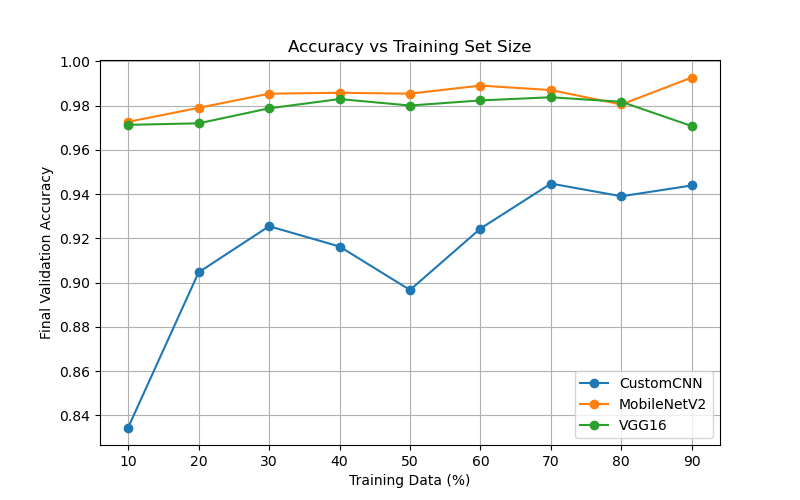
\includegraphics[width=0.6\textwidth]{img/acc_vs_split.png}
\caption{Celność każdego modelu dla rozmiaru zbioru treningowego.}
\label{fig:split}
\end{figure}

\section{CustomCNN}

\begin{figure}[H]
\centering
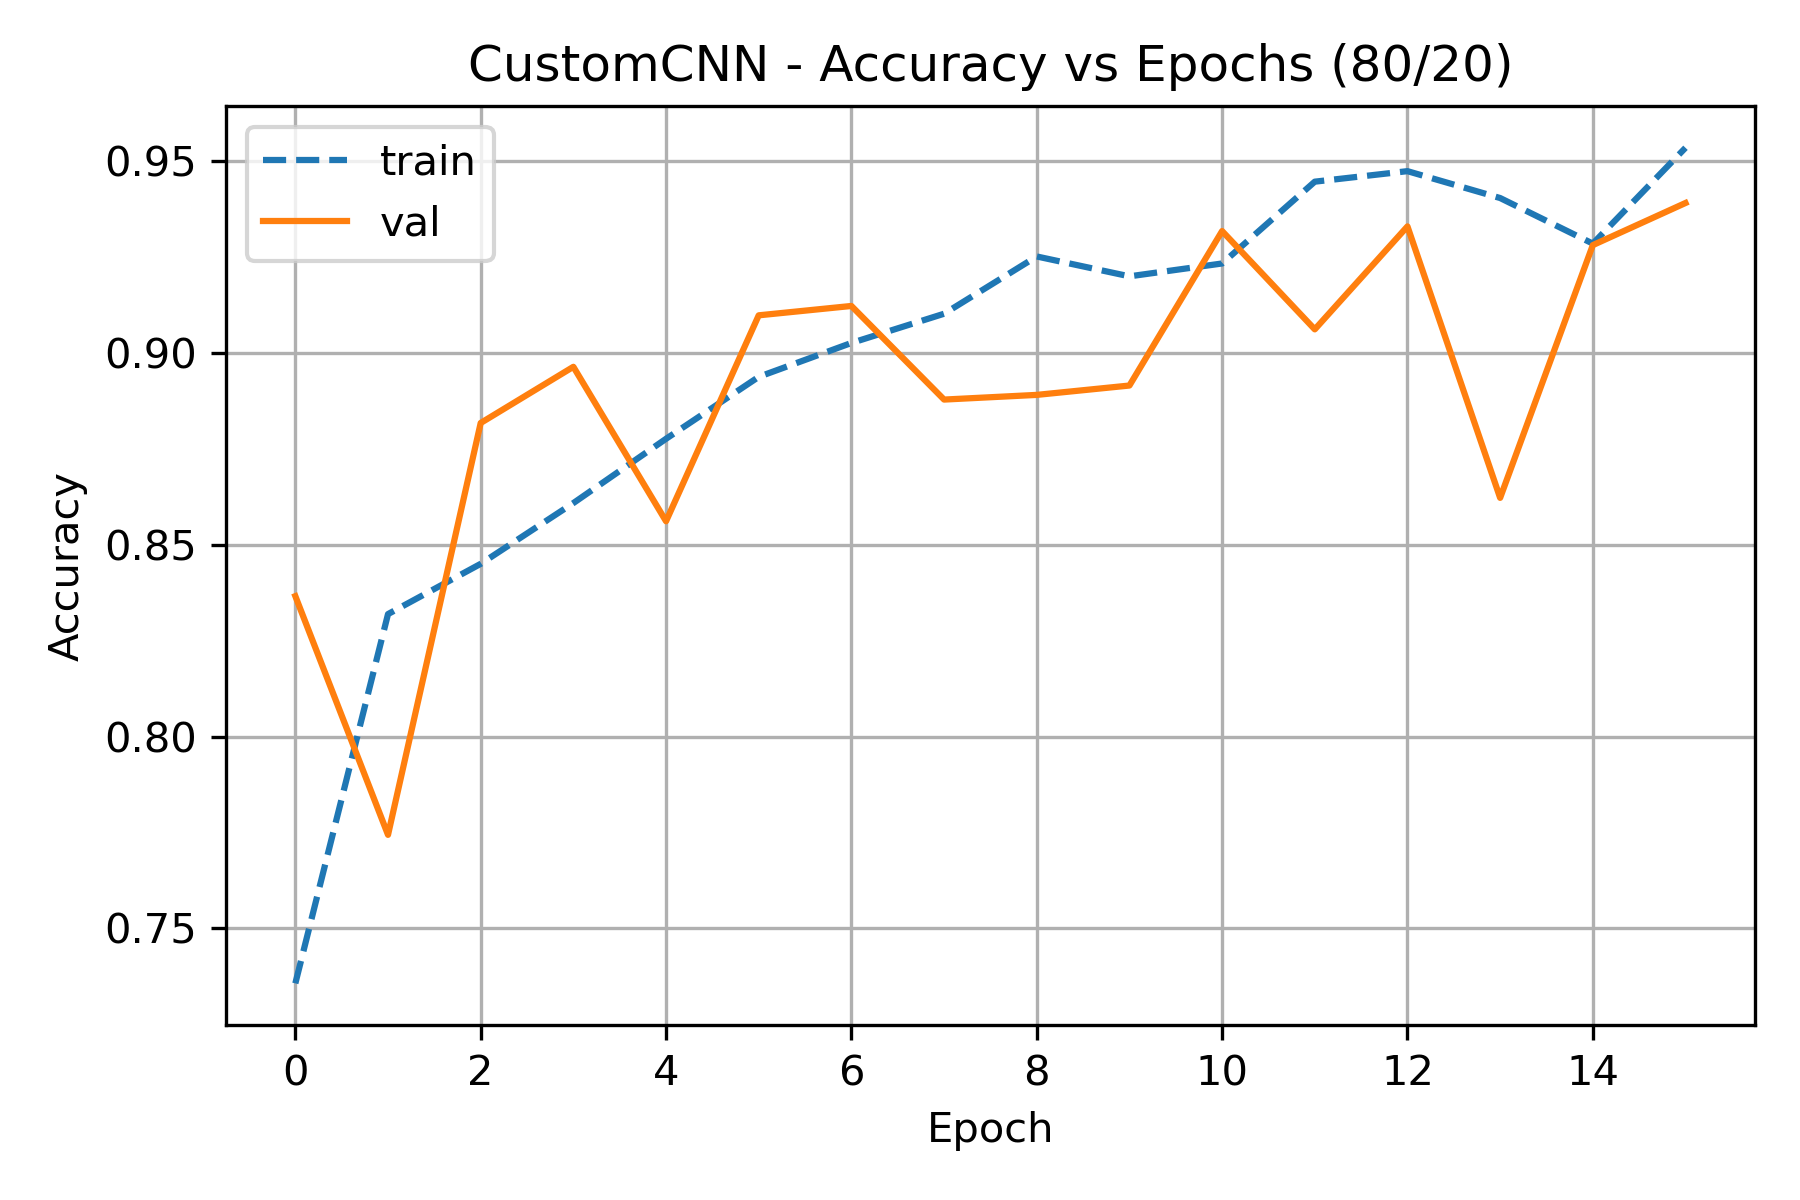
\includegraphics[width=0.6\textwidth]{img/acc_vs_ep_CustomCNN.png}
\caption{Celność modelu CustomCNN dla każdej epoki.}
\label{fig:customcnn_acc}
\end{figure}

\begin{figure}[H]
\centering
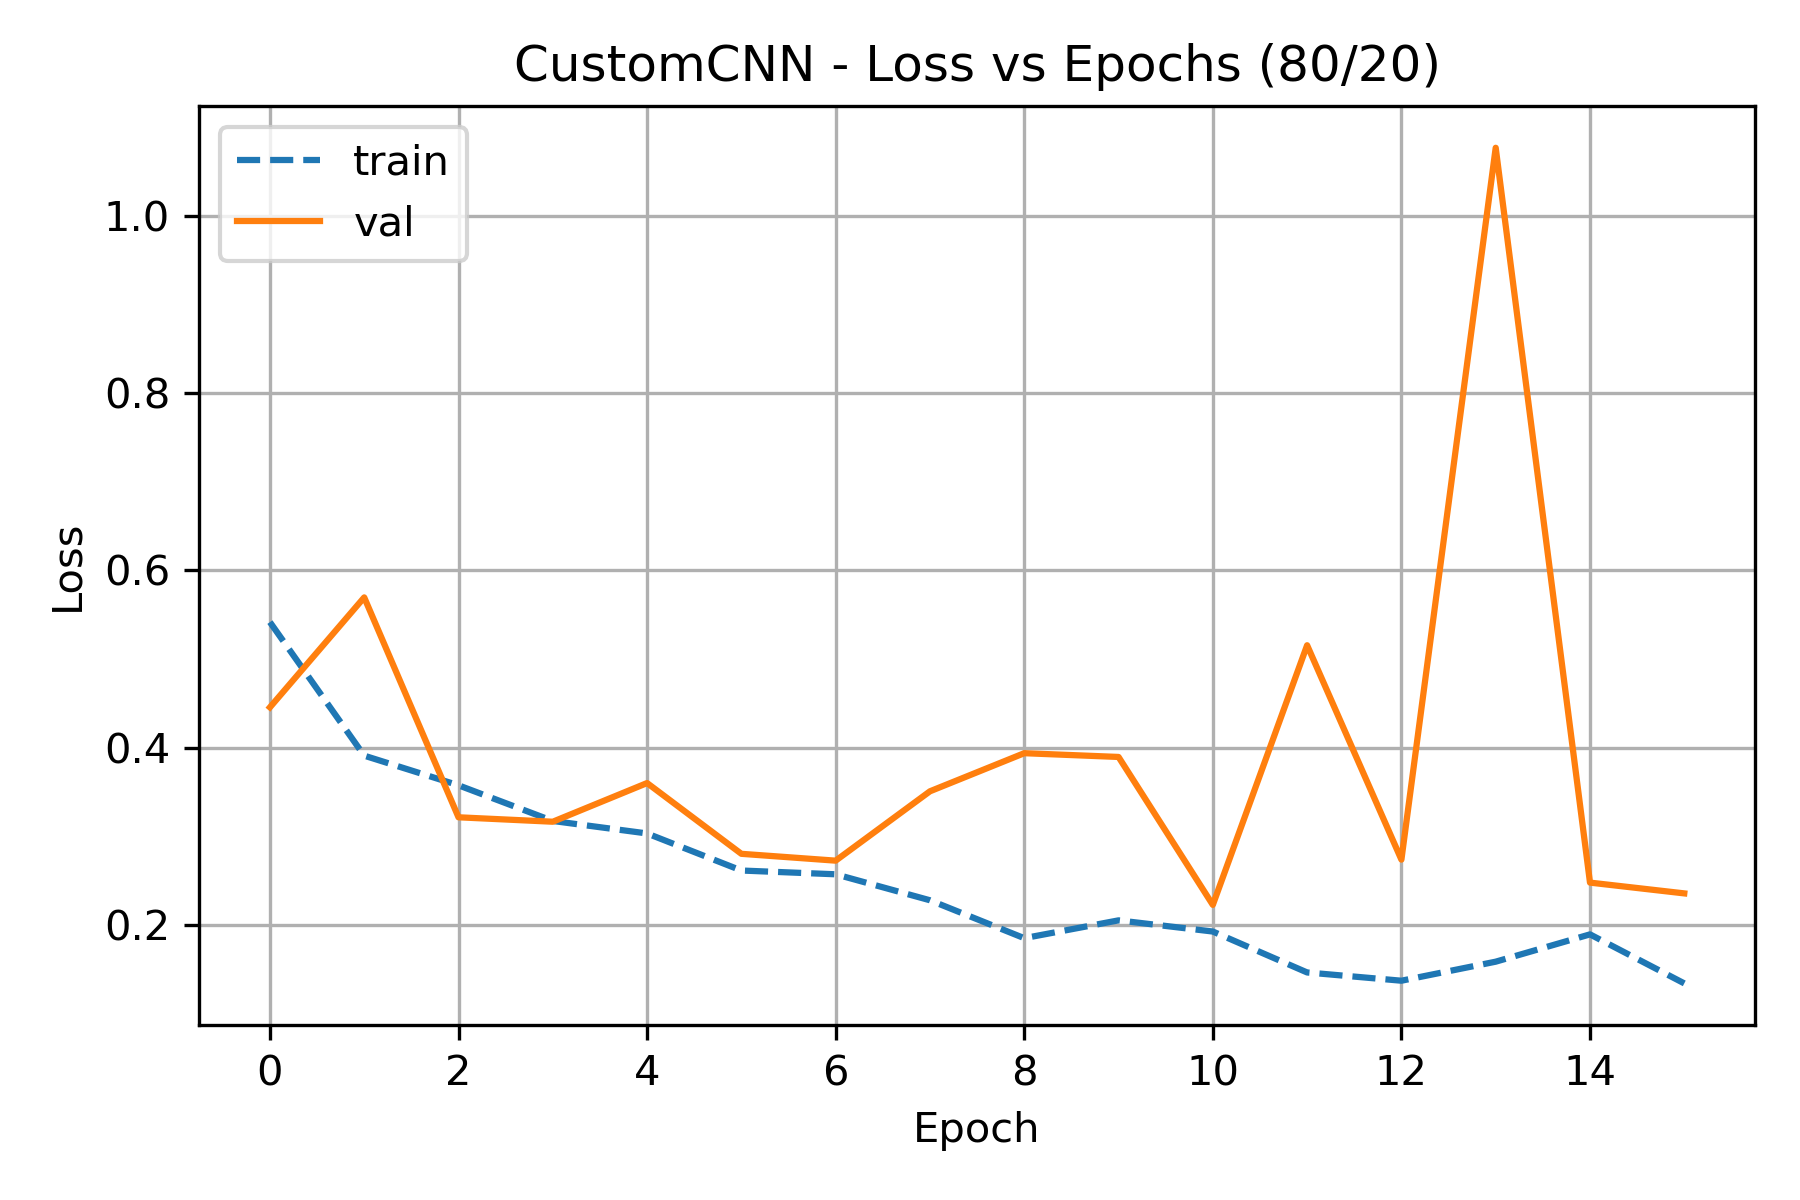
\includegraphics[width=0.6\textwidth]{img/loss_vs_ep_CustomCNN.png}
\caption{Loss modelu CustomCNN dla każdej epoki.}
\label{fig:customcnn_loss}
\end{figure}

\begin{figure}[H]
\centering
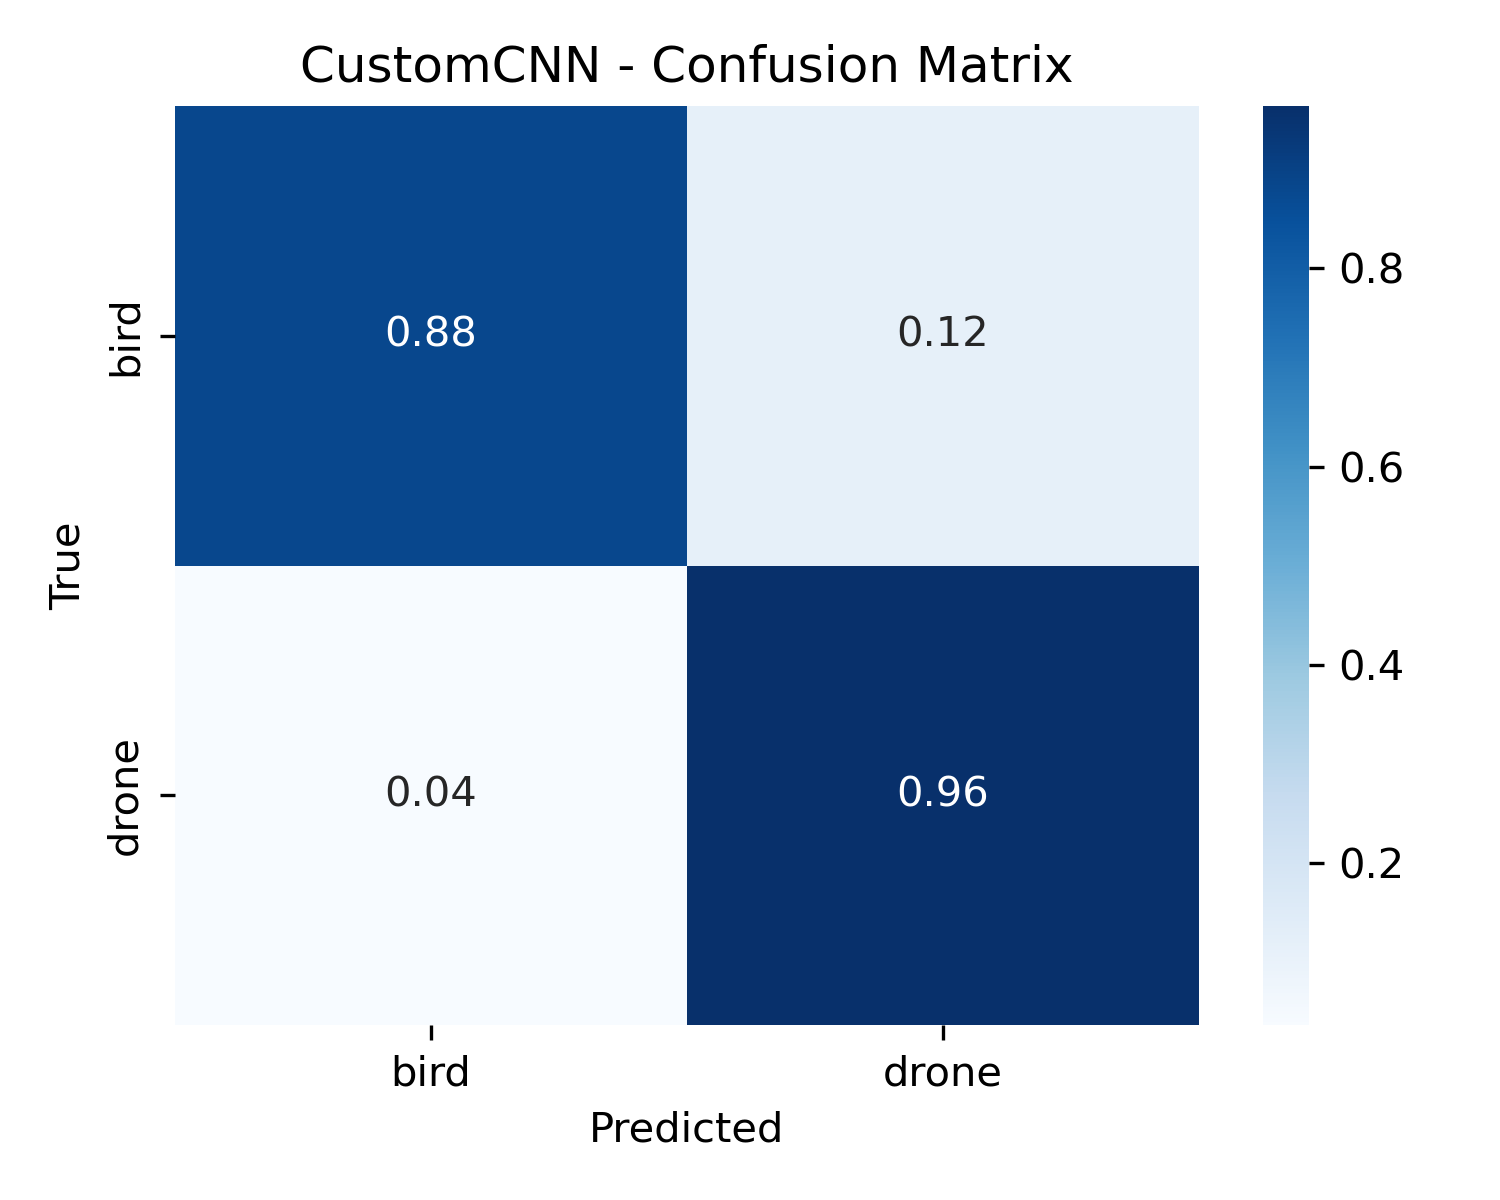
\includegraphics[width=0.6\textwidth]{img/conf_matrix_CustomCNN.png}
\caption{Macierz pomyłek modelu CustomCNN.}
\label{fig:customcnn_matrix}
\end{figure}

\section{MobileNetV2}

\begin{figure}[H]
\centering
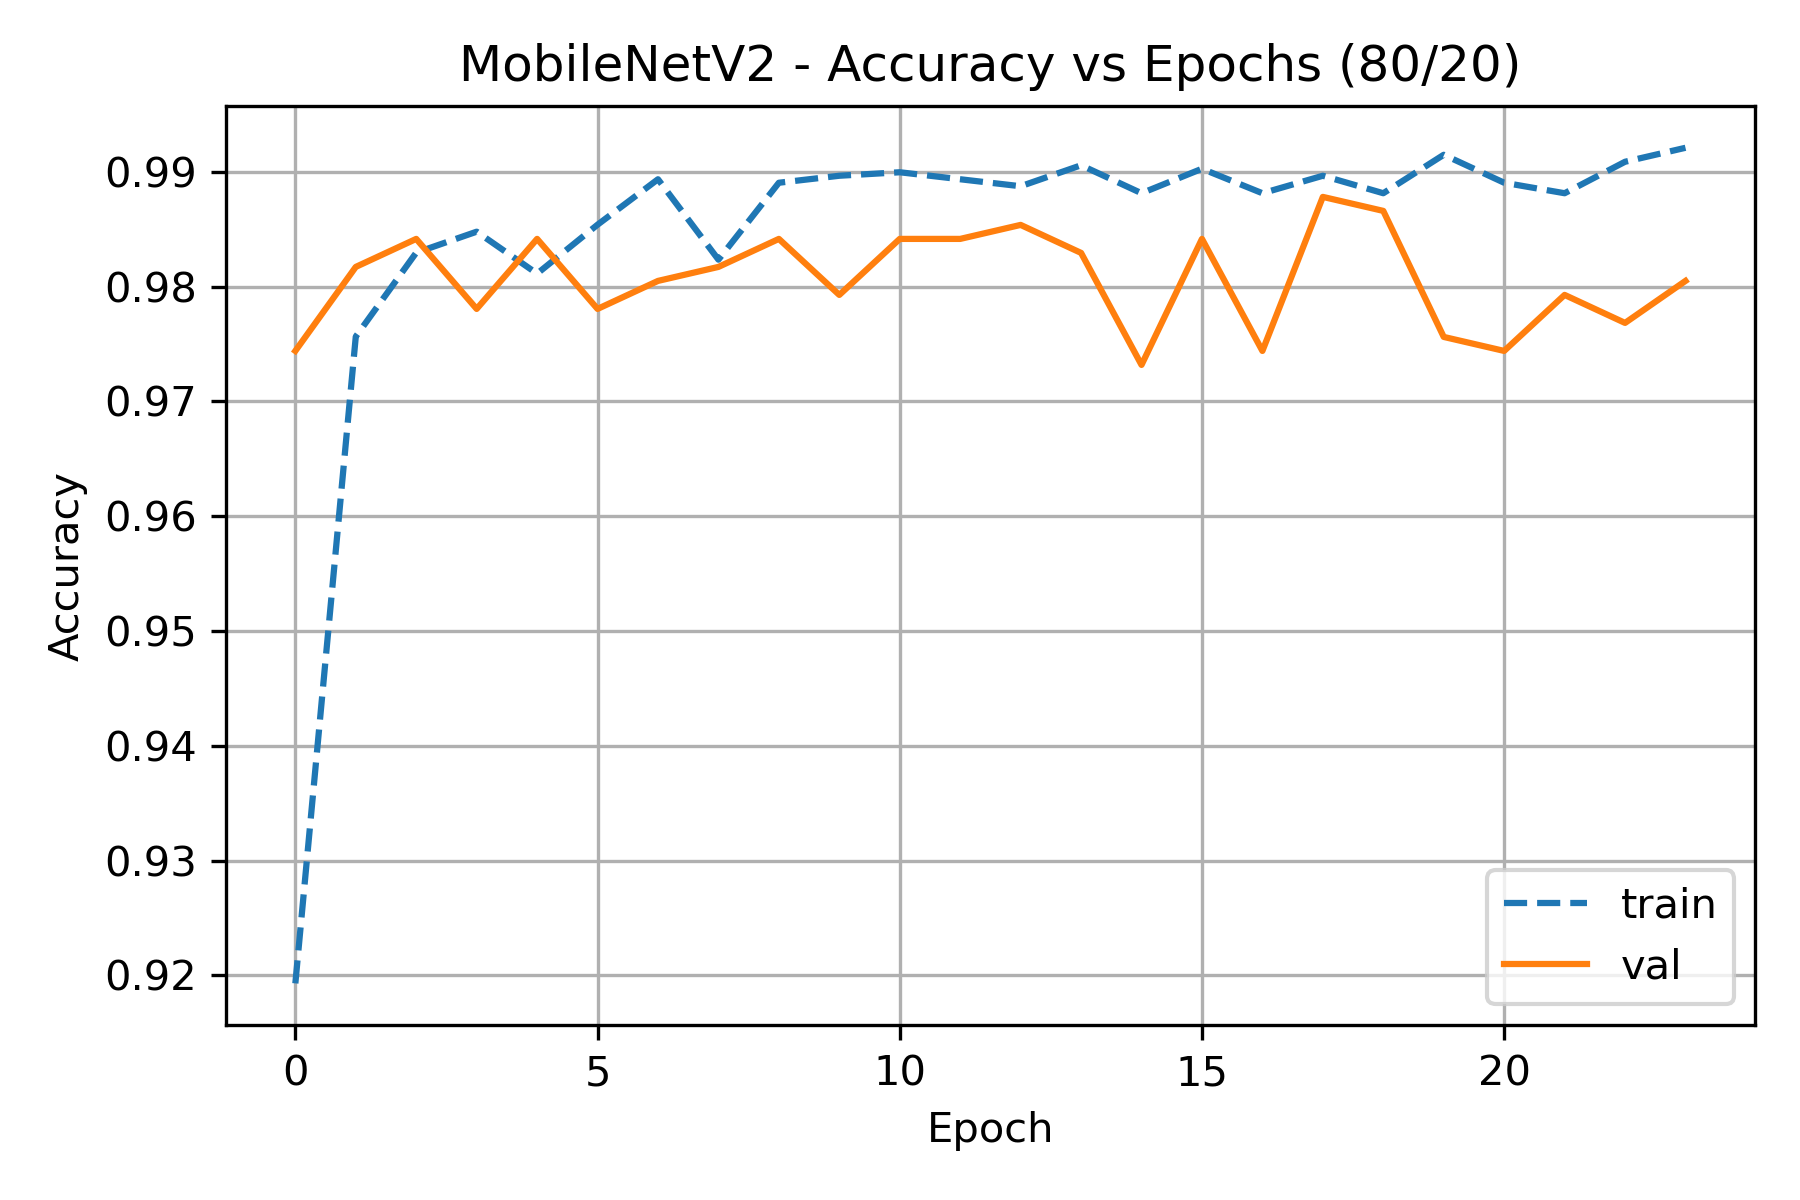
\includegraphics[width=0.6\textwidth]{img/acc_vs_ep_MobileNetV2.png}
\caption{Celność modelu MobileNetV2 dla każdej epoki.}
\label{fig:mobilenetv2_acc}
\end{figure}

\begin{figure}[H]
\centering
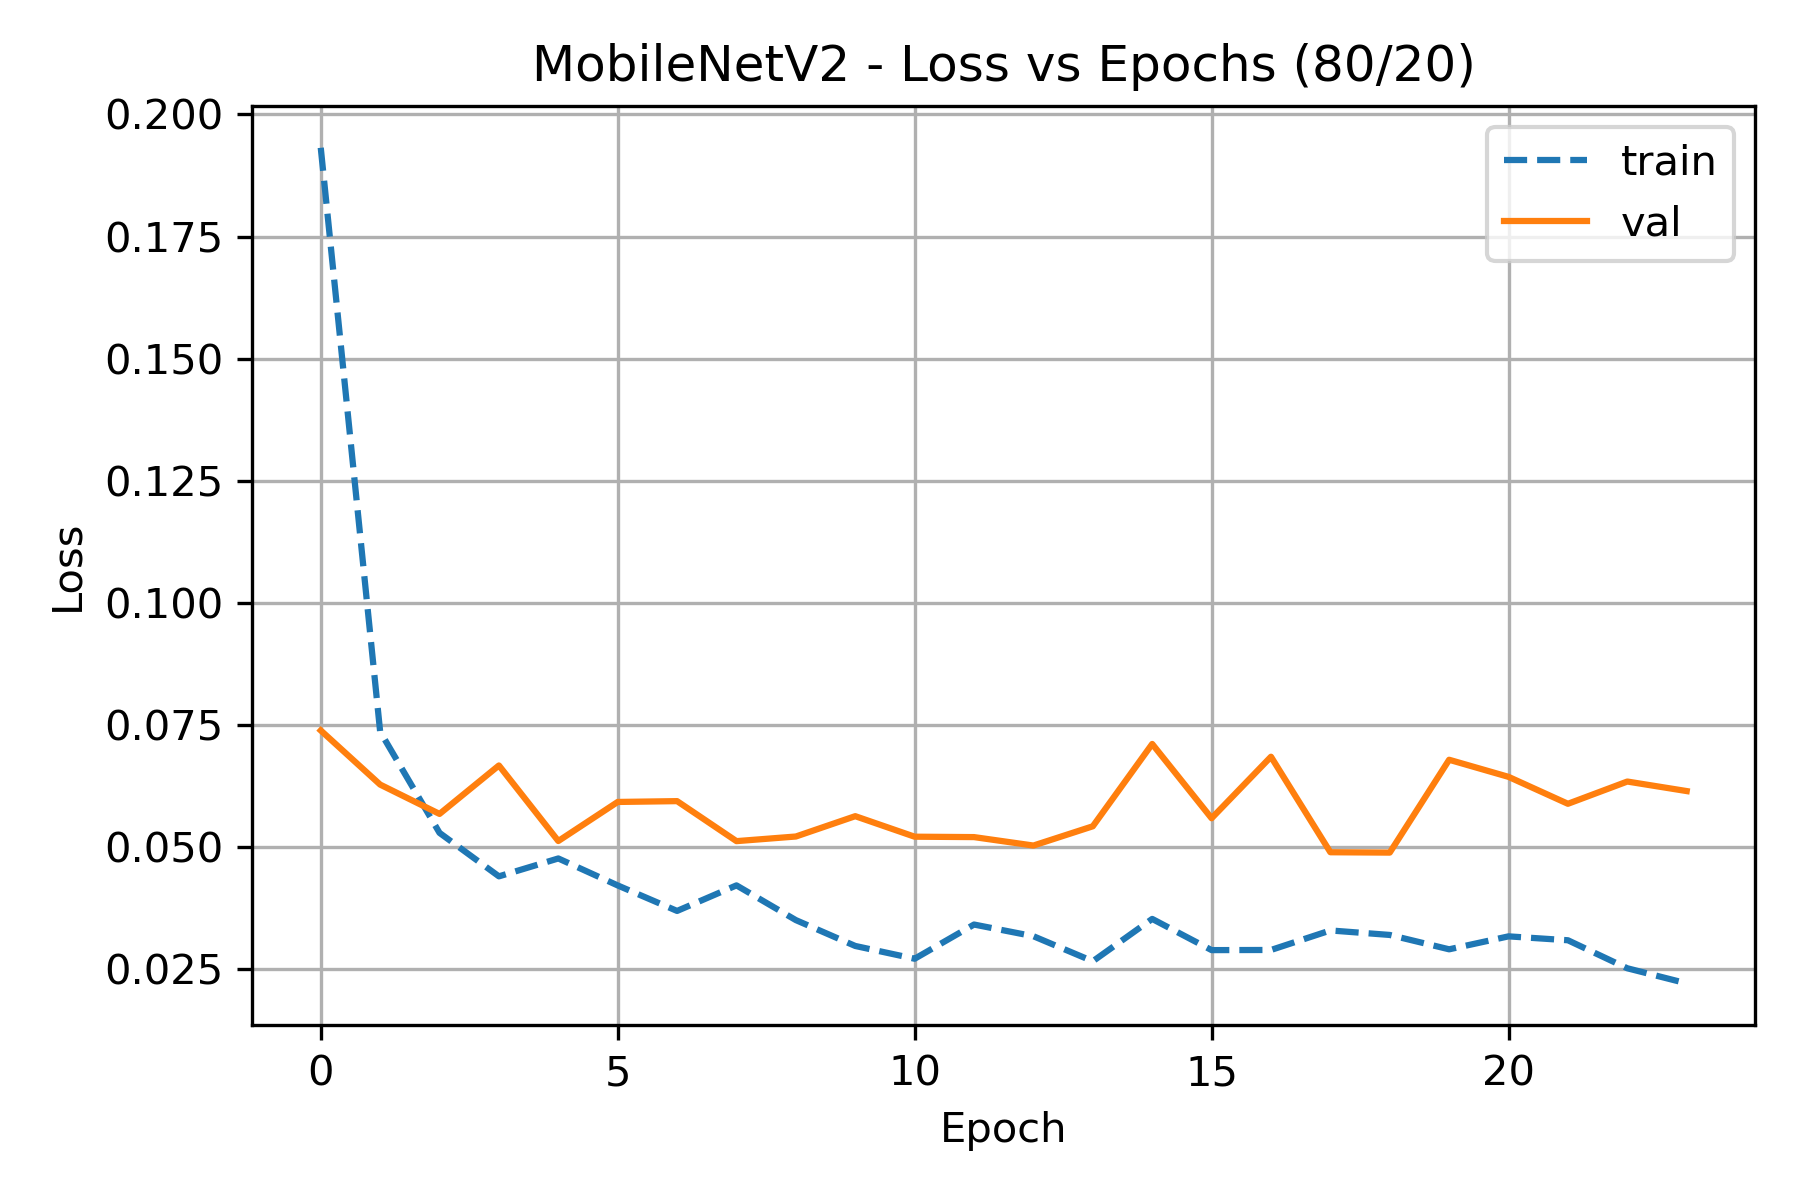
\includegraphics[width=0.6\textwidth]{img/loss_vs_ep_MobileNetV2.png}
\caption{Loss modelu MobileNetV2 dla każdej epoki.}
\label{fig:mobilenetv2_loss}
\end{figure}

\begin{figure}[H]
\centering
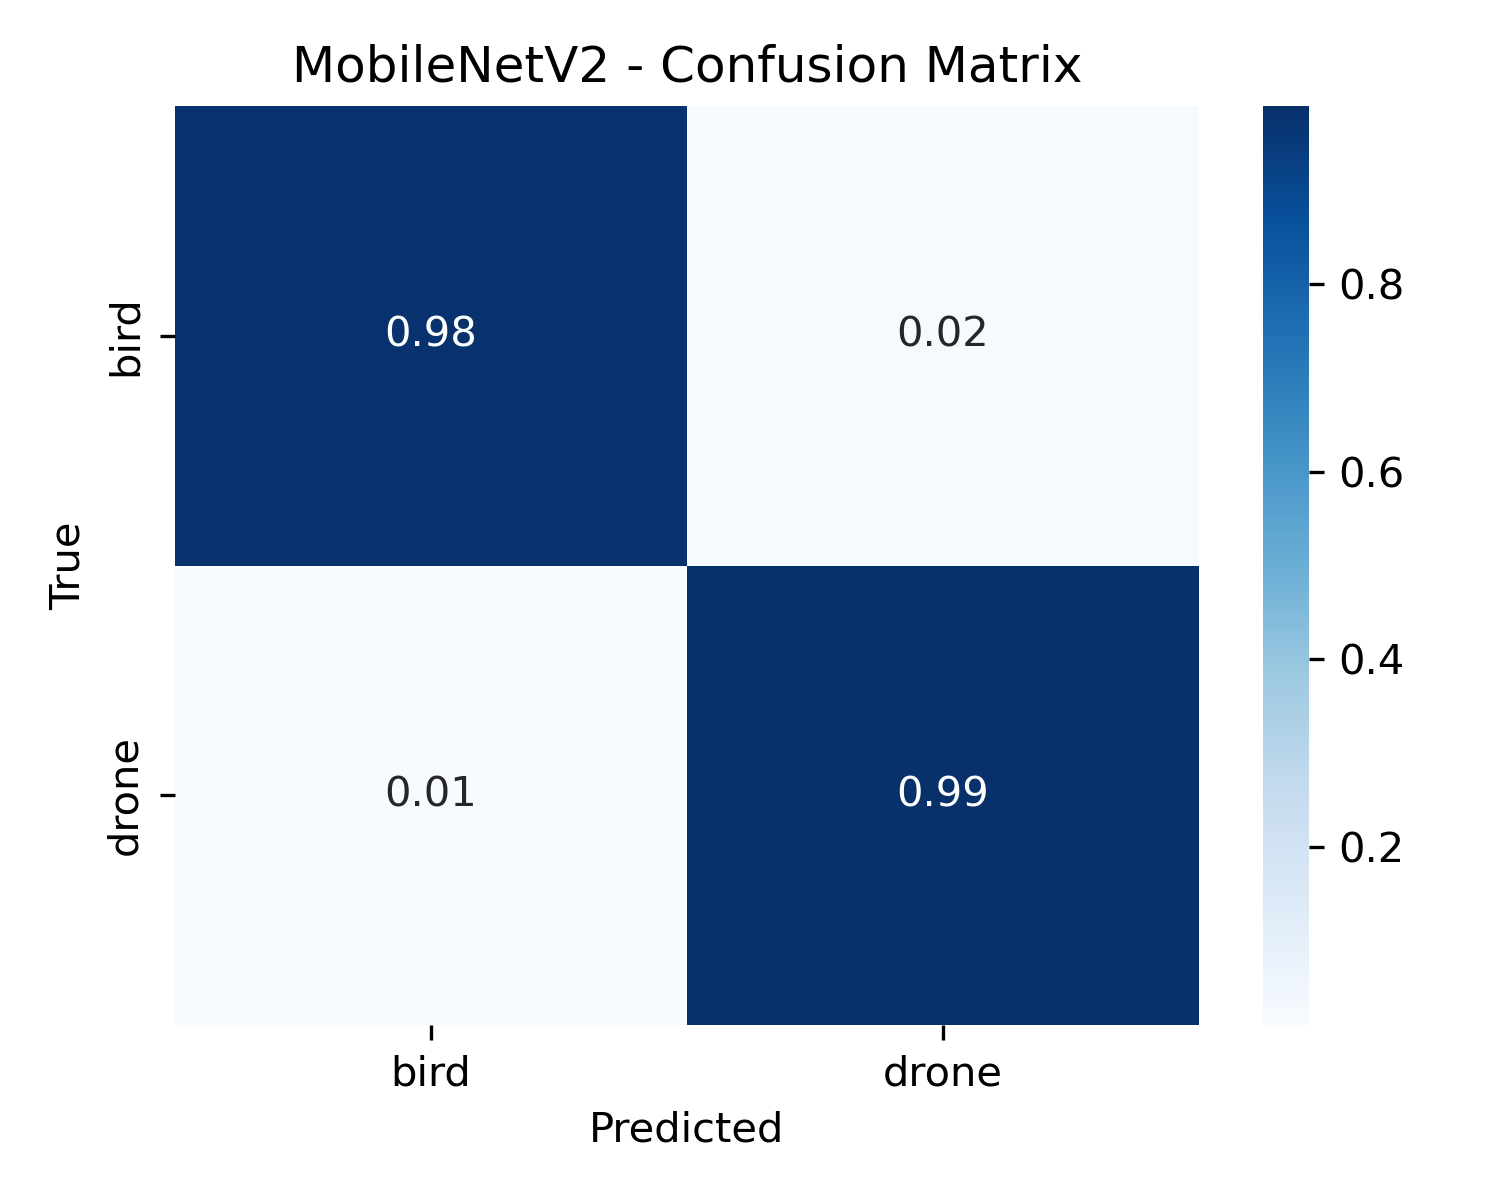
\includegraphics[width=0.6\textwidth]{img/conf_matrix_MobileNetV2.png}
\caption{Macierz pomyłek modelu MobileNetV2.}
\label{fig:mobilenetv2_matrix}
\end{figure}

\section{VGG16}

\begin{figure}[H]
\centering
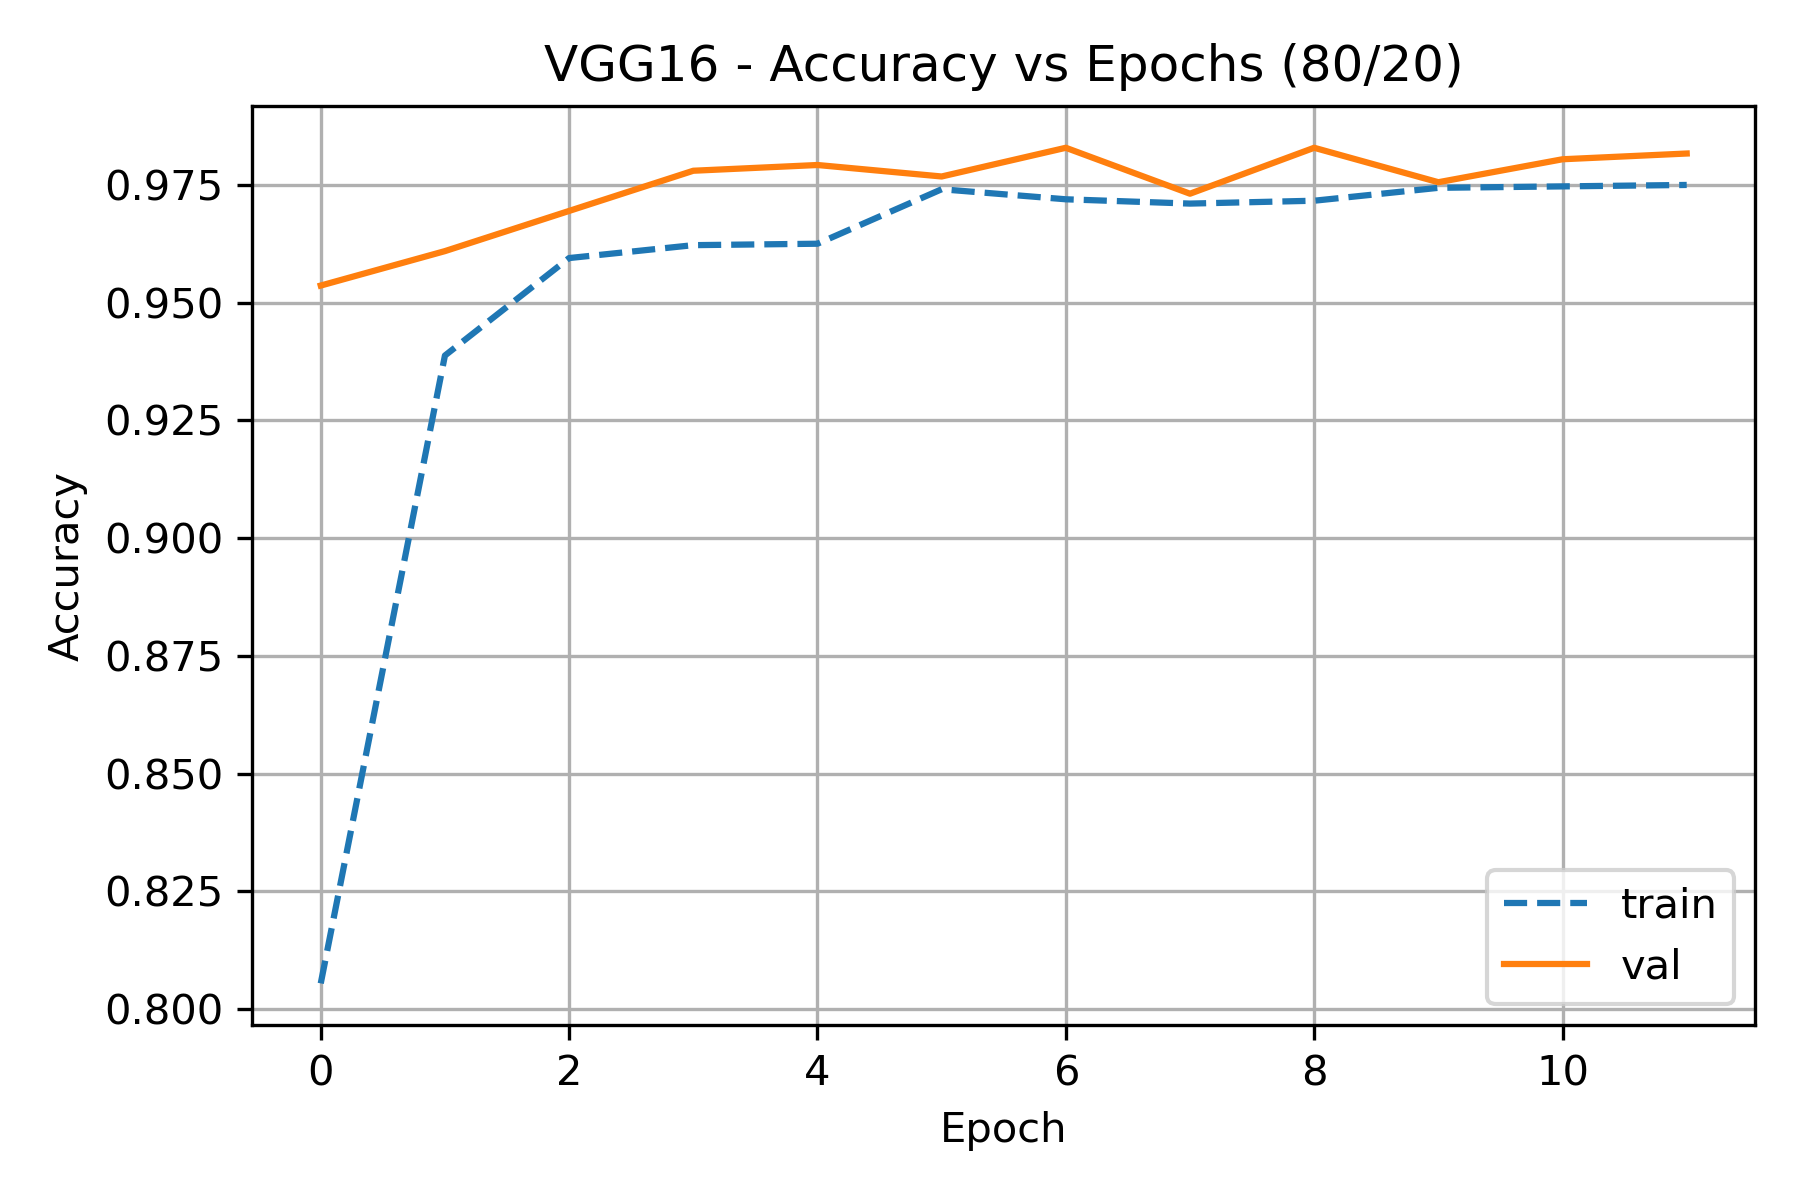
\includegraphics[width=0.6\textwidth]{img/acc_vs_ep_VGG16.png}
\caption{Celność modelu VGG16 dla każdej epoki.}
\label{fig:vgg16_acc}
\end{figure}

\begin{figure}[H]
\centering
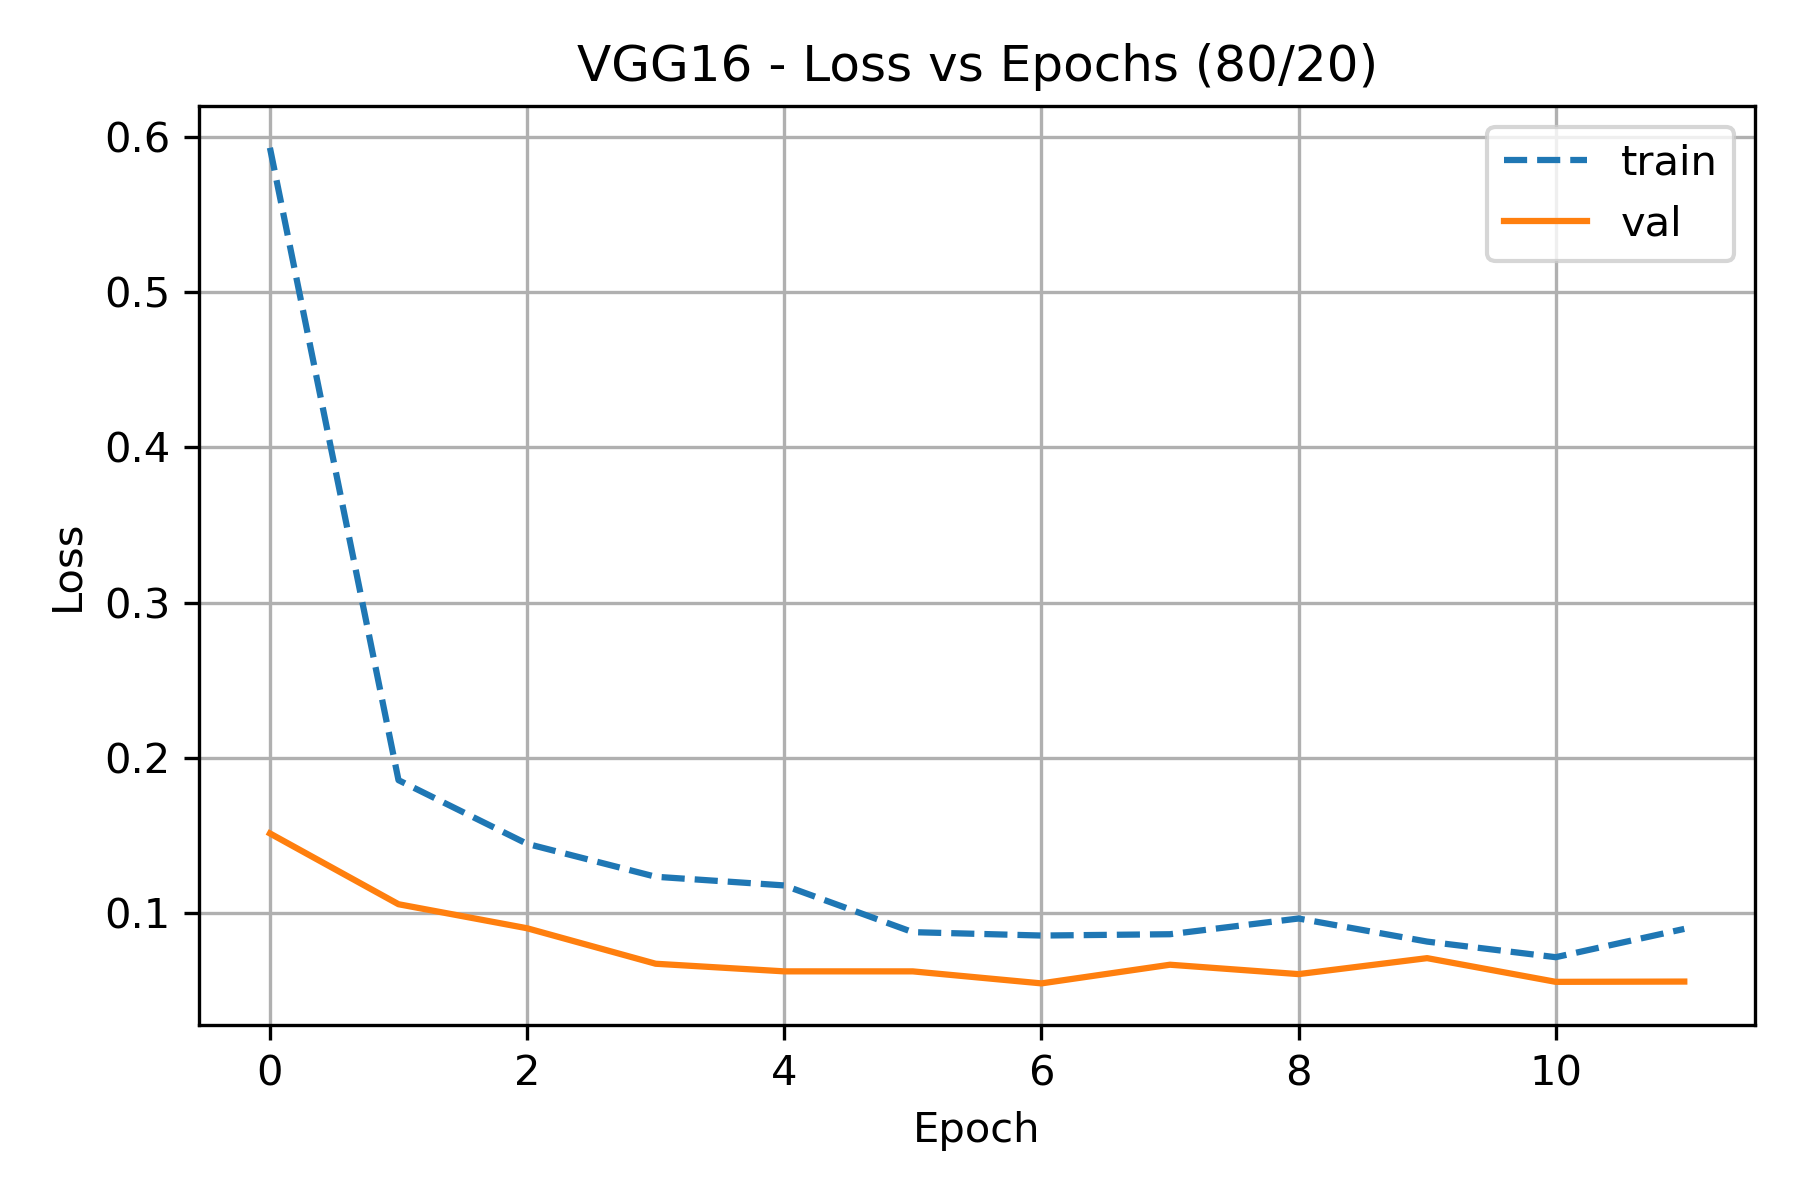
\includegraphics[width=0.6\textwidth]{img/loss_vs_ep_VGG16.png}
\caption{Loss modelu VGG16 dla każdej epoki.}
\label{fig:vgg16_loss}
\end{figure}

\begin{figure}[H]
\centering
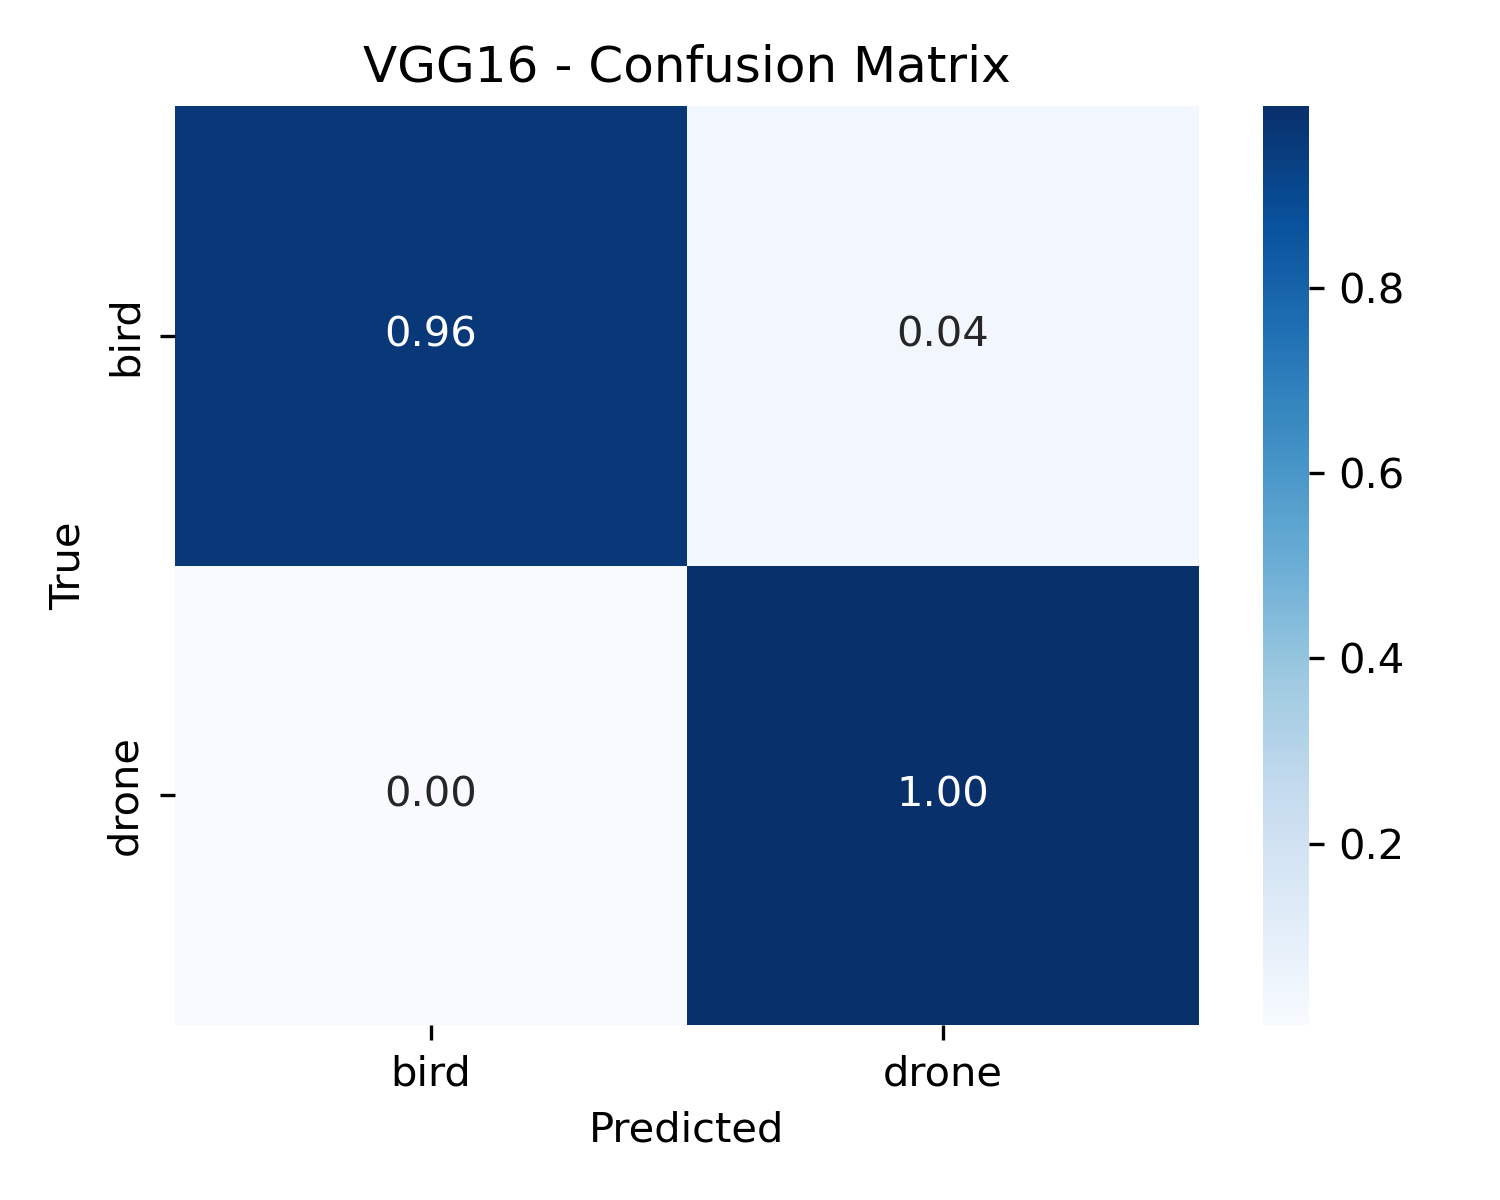
\includegraphics[width=0.6\textwidth]{img/conf_matrix_VGG16.png}
\caption{Macierz pomyłek modelu VGG16.}
\label{fig:vgg16_matrix}
\end{figure}

\chapter{Wnioski}

Na podstawie przeprowadzonych eksperymentów można stwierdzić, że wszystkie analizowane modele osiągnęły wysoką skuteczność w zadaniu klasyfikacji obrazów dronów i ptaków. Zarówno autorski model CustomCNN, jak i sieci prekonfigurowane MobileNetV2 oraz VGG16 uzyskały dobre wyniki w zakresie dokładności oraz pozostałych miar jakości klasyfikacji.

Modele wykorzystujące transfer learning wykazały nieznacznie lepszą skuteczność oraz stabilniejszy proces uczenia w porównaniu do modelu CustomCNN. Może to wynikać z faktu, że zostały one wcześniej wytrenowane na dużych i zróżnicowanych zbiorach danych, co pozwoliło im lepiej uogólniać cechy wizualne.

Jednym z czynników wpływających na ogólnie wysokie wyniki klasyfikacji może być stosunkowo niewielka liczba klas (dwie klasy), co upraszcza zadanie decyzyjne dla modeli. Dodatkowo, analiza danych wejściowych wskazuje, że obrazy ptaków często zawierają charakterystyczne cechy, takie jak rozpostarte skrzydła, które mogą być łatwo wykrywane przez sieci konwolucyjne jako istotne wzorce wizualne.

W przypadku klasy dronów część danych pochodziła z materiałów wideo, co mogło skutkować większą jednorodnością ujęć oraz podobieństwem między próbkami. Taka charakterystyka danych mogła dodatkowo ułatwić proces klasyfikacji i przyczynić się do uzyskania wysokich wartości metryk jakościowych.

Podsumowując, uzyskane wyniki potwierdzają skuteczność zastosowanych metod głębokiego uczenia w zadaniu klasyfikacji obrazów, jednocześnie wskazując na wpływ struktury danych oraz liczby klas na końcową jakość modeli.

\end{document}
